\section{Properties of Limits}

\begin{recap}
  \begin{itemize}
    \item If $f(x)$ is arbitrarily close to $L$ whenever $x$ is sufficiently close to, \textit{but not equal to} $a$, then we say $\dlim_{x\to a}f(x) = L$.
    \item If the left-side limit and the right-side limit do not match up, we say that the (two-sided) limit does not exist.
    \item We can estimate limits numerically by evaluating $f$ at $x$-values close to (and on either side of) $a$.
    We look to see if the $y$-values are arbitrarily close to some real number.
    \item We can estimate limits graphically by visualizing the function values around $a$, and again trying to see if the $y$-values are arbitrarily close to some value.
  \end{itemize}
\end{recap}

We've estimated limits numerically and graphically, but these can be difficult without more tools at our disposal.
Here we'll build up some analytic methods of evaluating limits.
We'll start by building some general limit laws for any function.

\subsection*{Limit Laws In General}

We will now think about functions in general, and build some laws/properties to apply to limits, no matter the context.
These properties will all be based around some basic operations on functions: addition, multiplication, division, and some exponents.

\begin{imp}{Limit Laws and Properties}
  Let $f$ and $g$ be two functions, and assume that $\dlim_{x\to a} f(x)$ and $\dlim_{x\to a} g(x)$ both exist.
  Then:
  \begin{enumerate}
    \item $\dlim_{x\to a} [f(x)\pm g(x)] = \lim_{x\to a} f(x) \pm \lim_{x\to a} g(x)$
    \item $\dlim_{x\to a} cf(x) = c\lim_{x\to a} f(x)$ for any constant multiple (coefficient) $c$.
    \item $\dlim_{x\to a} [f(x)\cdot g(x)] = \left[\lim_{x\to a} f(x)\right] \left[\lim_{x\to a} g(x)\right]$
    \item $\dlim_{x\to a} \frac{f(x)}{g(x)} = \frac{\dlim_{x\to a} f(x)}{\dlim_{x\to a} g(x)}$ if $\dlim_{x\to a} g(x)\neq0$
    \item $\dlim_{x\to a} (f(x))^n = \left(\dlim_{x\to a} f(x) \right)^n$ for integers $n$. (If $n<0$, there's actually division going on: make sure you don't divide by 0.)
  \end{enumerate}
\end{imp}

\begin{note}{Explanations}\hspace{1cm}
  \begin{enumerate}
    \item We should be able to rationalize this property, since $(f\pm g)(x)= f(x)\pm g(x)$.
    Since the limit is concerned with what the $y$-value is arbitrarily close to, we can see that the operation is ``preserved" across the limit.
    The following saying is helpful here: ``the limit of a sum (or difference) is the sum (or difference) of the limits.''
    \item Notice that a coefficient really represents repeated addition: $c\cdot f(x) = \underbrace{f(x) + f(x) + ...+ f(x)}_{c \text{ times}}$.
    \item ``The limit of a product is the product of the limits.''
    Limits preserve multiplication in the same way that they preserve sums.
    \item Dividing is really just multiplication by a reciprocal.
    The only thing we need to worry about is dividing by 0.\footnote{We'll investigate this more!}
    \item An exponent really represents repeated multiplication: $(f(x))^n = \underbrace{f(x) \cdot f(x) \cdot ... \cdot f(x)}_{n \text{ times}}$.
  \end{enumerate}
\end{note}

\subsection*{Examples}
Given $\dlim_{x\to 1} f(x) = 4$ and $\dlim_{x\to 1} g(x) = 2$, evaluate the following limits:
\begin{enumerate}
  \item $\dlim_{x\to 1}\left(\dfrac{f(x)-g(x)}{f(x)}\right)$

  When we consider $\dlim_{x\to 1}\left(\dfrac{f(x)-g(x)}{f(x)}\right)$, we should notice that the function $\dfrac{f(x)-g(x)}{f(x)}$ is really a combination of the two functions that we have information about.
  The operations are subtraction and division.
  We can use the properties above to re-write this limit:

  \begin{align*}
    \lim_{x\to 1}\left(\dfrac{f(x)-g(x)}{f(x)}\right) &= \frac{\dlim_{x\to 1} (f(x)-g(x))}{\dlim_{x\to 1} f(x)} & \text{Division Property (Property 4)}\\
    & = \frac{\left(\dlim_{x\to 1} f(x)\right)- \left(\dlim_{x\to 1} g(x)\right)}{\dlim_{x\to 1} f(x)} & \text{Difference Property (Property 1)}
  \end{align*}

  Now, we notice that we can input the values above, since we know that $\dlim_{x\to1} f(x) = 4$\footnote{Notice that since $\dlim_{x\to1}f(x)\neq0$, we're allowed to put this value in the denominator. Remember, we can't evaluate a limit using these properties if there's division by 0.} and $\dlim_{x\to 1}g(x) = 2$.

  \begin{align*}
    \frac{\left(\dlim_{x\to 1} f(x)\right)- \left(\dlim_{x\to 1} g(x)\right)}{\dlim_{x\to 1} f(x)} & = \frac{4-2}{4}\\
    &= \frac{2}{4} = \frac12
  \end{align*}

  So we can see that $\dlim_{x\to 1}\left(\dfrac{f(x)-g(x)}{f(x)}\right) = \frac{1}{2}$.

  \item $\dlim_{x\to 1} \left(3f(x)+\dfrac{2(g(x))^3}{5}\right)$

  Here, we have two functions added together, an exponent on one, and coefficients on each. We can again use the properties above.
  Again, we'll use the properties above:

  \begin{align*}
    \dlim_{x\to 1} \bigg( 3f(x) &\left.+\dfrac{2(g(x))^3}{5}\right) \\
    & = \left(\dlim_{x\to 1} 3f(x)\right) + \left(\dfrac{2(g(x))^3}{5}\right) & \text{Sum Property (Property 1)}\\
    &= 3\left(\dlim_{x\to 1} f(x)\right) + \dfrac{2}{5}\left(\dlim_{x\to1} (g(x))^3 \right) & \text{Coefficient Property (Property 2)}\\
    & = 3\left(\dlim_{x\to 1} f(x)\right) + \dfrac{2}{5}\left(\dlim_{x\to 1}g(x)\right)^3 & \text{Exponent Property (Property 5)}
  \end{align*}

  Again, we can input the values above, since $\dlim_{x\to1} f(x) = 4$ and $\dlim_{x\to 1}g(x) = 2$ are given.

  \begin{align*}
    3\left(\dlim_{x\to 1} f(x)\right) + \dfrac{2}{5}\left(\dlim_{x\to 1}g(x)\right)^3 & =3(4) + \dfrac{2}{5}(2)^3 \\
    &= 12 + \dfrac{2}{5}(8) = 12 + \dfrac{16}{5}\\
    & = \dfrac{76}{5}
  \end{align*}

  So the limit $\dlim_{x\to 1} \left(3f(x)+\dfrac{2(g(x))^3}{5}\right) = \dfrac{76}{5}$.
\end{enumerate}

We can see that these limit laws are very helpful for building our limit ``piece-by-piece.''
What happens, though, when we have some function or combination of functions that involves an operation or function type that is not covered in these properties?

One last thing to think about is a more generlized property for exponents.
Our property above only holds for integer exponents.
\begin{note}{Remember}
  Roots and radicals can be written as fraction exponents.
  \[\sqrt{x} = x^{1/2}\]
\end{note}

\subsection*{Square Roots}

Let's consider the function $y=\sqrt{x}$.
Specifically, we'll consider $\dlim_{x\to 0} \sqrt{x}$.

In the spirit of this chapter, we should start with numerical and graphical esimations.

\subsubsection*{Graphical Approximation}

Let's consider the graph of $y=\sqrt{x}$ around $x=0$.

\begin{figure}
  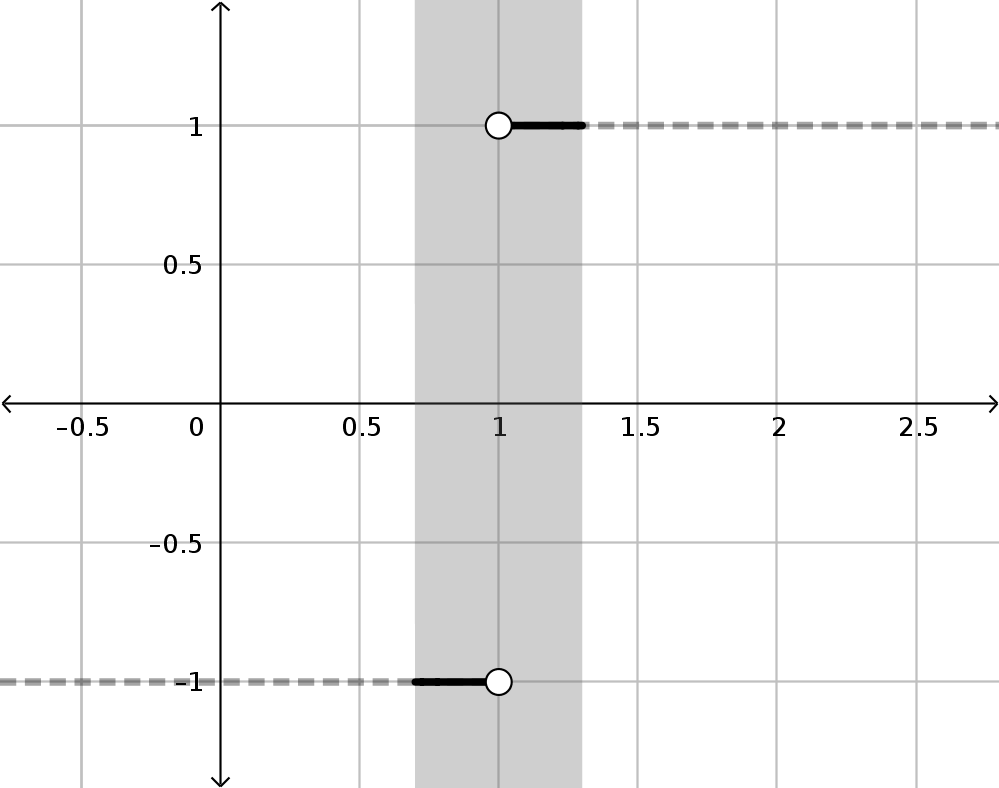
\includegraphics[scale=0.5]{./1_limits/images/1-2_graph3.png}
  \centering
\end{figure}



\subsubsection*{Numerical Approximation}

\textbf{Left-Sided Limit}

\begin{tabular}{ccccc} \toprule
  $\bm{x}$ & $-0.5$ & $-0.1$ & $-0.01$ & $-0.001$ \\ \midrule
  $\bm{\sqrt{x}}$ & $\sqrt{-0.5}$ & $\sqrt{-0.1}$ & $\sqrt{-0.01}$ & $\sqrt{-0.001}$\\ \bottomrule
\end{tabular}

\begin{flushright}
  \textbf{Right-Sided Limit}

  \begin{tabular}{ccccc} \toprule
    $0.001$ & $0.01$ & $0.1$ & $0.5$ & $\bm{x}$ \\ \midrule
    $\sqrt{0.001}$ & $\sqrt{0.01}$ & $\sqrt{0.1}$ & $\sqrt{0.5}$ & $\bm{\sqrt{x}}$ \\ \bottomrule
  \end{tabular}
\end{flushright}

We should notice the strange behavior here, specifically with the left-sided limit.

None of those outputs are real numbers.
Strange.

On a different note, the right-sided limit looks like it's approaching 0, whether we're thinking about the graphical approximation or the numerical approximation.
